%2021_05_28
\paragraph{Parametri amperspire}
Si applica la legge di Ampère ad un circuito magnetico con traferro sul quale è avvolto
un avvolgimento di $N$ spire
$$
\oint_\Gamma \vec{H}\cdot\hat{t}dl = Ni
$$

Fissata l'induzione desiderata e la tensione di alimentazione, si vuole 
determinare il numero di spire $N$ necessarie e conseguentemente la corrente 
$i$ che le attraverserà.

La resistenza dell'avvolgimento è 
$$
R = N\cdot \eta\frac{l}{A}
$$

Si trascura l'autoinduzione dell'avvolgimento se questo è alimentato da tensione continua.
Considerata dunque la legge di Ohm
$$
v = Ri = Ni\eta\frac{l}{A} \Rightarrow v = Ni \eta \frac{l}{A}
$$
Fissata la tensione di alimentazione si possono ricavare i parametri $N$ ed $i$ o viceversa.

\subsection{Magneti permanenti}
Prevedono applicazioni in molti campi come nei moderni motori elettrici brushless.
È possibile invece utilizzare i magneti permanenti per realizzare degli attuatori
elettromeccanici.

Data una regione $\Omega$ e sia $\vec{M}(p')\ p'\in\ \Omega$ il campo di magnetizzazione
all'interno del dominio, si vuole calcolare il campo $\vec{B}$ o $\vec{H}$ prodotto
in assenza di correnti (libere).
\begin{figure}[H]
\centering
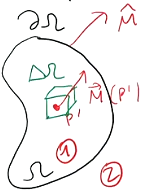
\includegraphics[width = 0.2\linewidth]{magnete_permanente}
\end{figure}
Le equazioni di campo sono
$$
\begin{aligned}
&\nabla\cdot\vec{B} = 0\qquad\qquad\qquad\  \text{in }\Omega \text{ punti regolari} \\
&\nabla\times\vec{H} =  0\\
&\hat{n}\cdot\left(\vec{B}_2-\vec{B}_1\right) = 0\qquad\ \ \text{continuità di }\vec{B}\cdot\hat{n}\text{ su }\partial\Omega \\
&\hat{n}\times\left(\vec{H}_2-\vec{H}_1\right) = 0\qquad \text{continuità di }\hat{n}\times\vec{H}\text{ su }\partial\Omega\\
&\vec{B} = \mu_0\left(\vec{H}+\vec{M}\right)
\end{aligned}
$$

Nell'ipotesi di magnete permanente, si assume assegnato il campo $\vec{M}$. Se si suppone il 
dominio a connessione semplice e il rotore $\nabla\times\vec{H}=0$ allora è possibile
definire una funzione potenziale scalare per il campo $\vec{H}$. Si sostituisce
l'equazione del campo $\vec{B}$ nell'equazione che contiene la sua divergenza e si pone
$\vec{H}= \vec{H}_m$ perché prodotto dalla sola magnetizzazione e non da correnti libere.
Le equazioni del sistema diventano:
$$
\begin{aligned}
&\nabla\cdot\left(\mu_0\vec{H}_m\right) = - \nabla\cdot\left(\mu_0\vec{M}\right)
\Rightarrow \nabla\cdot\vec{H}_m = -\nabla\cdot\vec{M}\\
&\nabla\times\vec{H}_m=0\\
&\hat{n}\cdot\left(\mu_0\vec{H}_{m_2} + \mu_0\vec{M}_2 - \mu_0\vec{H}_{m_1}-\mu_0\vec{M}_1\right) = 0\\
&\hat{n}\times\left(\vec{H}_{m_2}-\vec{H}_{m_1}\right) = 0
\end{aligned}
$$
Se si considera la regione magnetizzata come regione (1) e il vuoto come regione (2)
si ha che $\vec{M}_2 = 0$ dato che la magnetizzazione risiede solo nella materia.

Riscrivendo si ottiene
$$
\begin{aligned}
&\nabla\cdot\vec{H}_m = -\nabla\cdot\vec{M}\\
&\nabla\times\vec{H}_m = 0\\
&\hat{n}\cdot\left(\vec{H}_{m_2}-\vec{H}_{m_1}\right) = \hat{n}\cdot\vec{M}
\end{aligned}
$$
Il campo $\vec{H}_m$ viene chiamato campo demagnetizzante prodotto dalla
magnetizzazione. Lo si confronta invece con il campo elettrostatico generato 
da una superficie carica al suo interno da una carica $\rho$ e sulla superficie da 
una carica superficiale $\sigma$.
Le equazioni del campo elettrostatico sono
$$
\begin{aligned}
&\nabla\cdot\vec{E} = \frac{\rho}{\varepsilon_0} \\
&\nabla\times\vec{E} = 0\\
&\hat{n}\cdot\left(\vec{E}_2-\vec{E}_1\right) = \frac{\sigma}{\varepsilon_0}
\end{aligned}
$$
I due set di equazioni sono matematicamente uguali a patto di considerare delle 
distribuzioni di cariche magnetiche equivalenti, che nella realtà non esistono. 
$$
\begin{aligned}
&\rho_m = -\nabla\cdot\vec{M}\\
&\sigma_m = \hat{n}\cdot\vec{M}
\end{aligned}
$$
Queste cariche definiscono il cosiddetto approccio Coulombiano al campo magnetico, quello
utilizzato in precedenza, a partire dalle correnti molecolari è stato invece l'approccio
Amperiano.
$$
\begin{aligned}
&\vec{J}_\text{mol} = \nabla\times\vec{M} \\
&\vec{J}_{S\text{ mol}} = \vec{M}\times\hat{n}
\end{aligned}
$$
Questi due approcci sono duali.
\newpage
Nel caso dei magneti permanenti l'approccio Coulombiano necessita della risoluzione di un'equazione di Poisson scalare, mediante la soluzione del potenziale scalare.
Viceversa nell'approccio Amperiano è necessario risolvere un'equazione vettoriale riferita
ad un potenziale vettore.
Risulta evidente la convenienza del primo approccio dovuto al minor numero di equazioni.

\paragraph{Campo $\vec{H}_m$ e $\vec{B}$ prodotto da un magnete cilindrico}
Si supponga di avere un magnete cilindrico magnetizzato uniformemente lungo l'asse.
\begin{figure}[H]
\centering
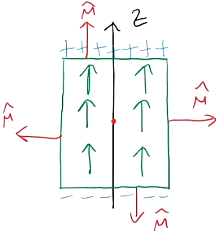
\includegraphics[width=0.3\linewidth]{magnete_permanente_cilindrico}
\end{figure}
Le cariche magnetiche sono:
$$
\rho_m = \nabla\cdot\vec{M} = 0
$$
poiché la magnetizzazione è costante, la sua divergenza è nulla, quindi non ci sono
cariche di volume ma solo cariche superficiali
$$
\sigma_m = \vec{M}\cdot\hat{n}
$$
Il prodotto scalare come si evince dalla geometria è nullo sulle superfici laterali,
ciò implica che le cariche superficiali sono necessariamente localizzate sulle
superfici superiori e inferiori del cilindro con segno concorde al segno del prodotto 
scalare tra campo e normale alla superficie.

Il campo magnetico equivale ad un campo elettrostatico generato da due 
armature ``a disco''.

È quindi intuitivo rappresentare le linee di campo in analogia a quello elettrostatico.
Le linee sono discontinue rispetto alla normale delle superfici cariche.
\begin{figure}[H]
\centering
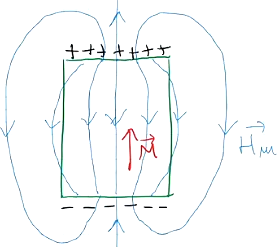
\includegraphics[width = 0.3\linewidth]{magnete_permanente_linee_campo}
\end{figure}

La discontinuità presente sulle superfici cariche è pari a
$$
\hat{n}\cdot\left(\vec{H}_{m_2}-\vec{H}_{m_1}\right) = \vec{M}\cdot\hat{n}
$$
ossia alla magnetizzazione del corpo
$$
\vec{e}_z \cdot \left(\vec{H}_{m_2}-\vec{H}_{m_1}\right) = M_0
$$

Il campo $\vec{H}_m$ viene chiamato demagnetizzante perché è diretto in verso opposto
rispetto alla magnetizzazione, è un campo che cerca di minimizzare o ridurre la 
magnetizzazione.

Il fenomeno della minimizzazione della magnetizzazione genera ad esempio in una struttura
piana un dominio a forma di busta da lettera come mostrato in figura.
\begin{figure}[H]
\centering
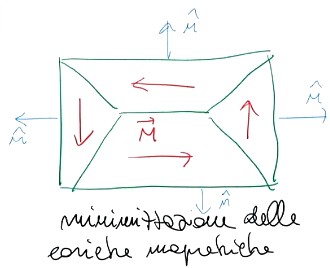
\includegraphics[width = 0.4\linewidth]{minimizzazione_magnetizzazione}
\end{figure}
Le cariche di volume sono nulle all'interno dei singoli domini a causa
della magnetizzazione costante e le cariche superficiali sono nulle
sulla frontiera esterna perché il campo di magnetizzazione non ha una componente
normale alla stessa.

Sono invece presenti cariche solo sulle frontiere interne o regioni di transizione
tra i domini orientati diversamente tra loro dato che la divergenza non potrà essere
nulla su queste regioni.

Si ha la configurazione di Landau e il minimo quantitativo di cariche magnetiche se il 
dominio è quadrato.

Un caso diverso se la magnetizzazione è circolare, a vortice, si ha una regione al centro 
della geometria chiamata ``vortex core'' in cui la magnetizzazione è esterna al piano.
\begin{figure}[H]
\centering
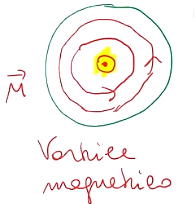
\includegraphics[width = 0.3\linewidth]{vortice_magnetico}
\end{figure}
\newpage

\subparagraph{Analisi del campo $\vec{B}$ in un magnete permanente}
Per il campo $\vec{B}$ è utile considerare la trattazione Amperiana, si analizzano dunque
le correnti molecolari.
All'interno del dominio non sono presenti correnti dato che il rotore è nullo
$$
J_{\text{mol}} = \nabla\times\vec{M} = 0
$$
Le correnti superficiali amperiane sono invece pari a 
$$
\vec{J}_{S\text{ mol}} = \vec{M}\times\hat{n}
$$
sono nulle dunque sulle facce superiore e inferiore, mentre diverse da zero sulle superfici
laterali del dominio, in maniera del tutto duale rispetto al campo $\vec{H}_m$ e 
alle cariche magnetiche.

È come se l'intero cilindro fosse circondato da correnti che percorrono la sua superficie
laterale, orientate con la regola della mano destra rispetto al vettore magnetizzazione
e normale alla superficie, come mostrato in figura.
\begin{figure}[H]
\centering
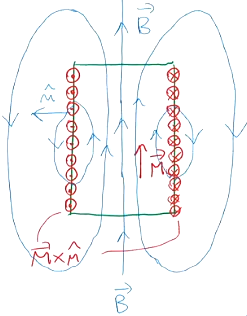
\includegraphics[width = 0.3\linewidth]{magnetizzazione_cilindro_campo_B}
\end{figure}

È prossimo al campo di un solenoide finito di altezza $h$, ha un asse di simmetria
in cui $\vec{B}$ è perfettamente allineato all'asse $z$ e linee che concatenano le correnti.

È interessante studiare il campo all'avvicinarsi della frontiera laterale, vale la 
discontinuità della tangente di $\vec{B}$
$$
\hat{n}\times\left(\vec{B}_2-\vec{B}_1\right) = \vec{J}_{S\text{ mol}}
$$
Le linee in prossimità della superficie laterale dunque la attraversano formando un angolo
e richiudendosi dall'esterno.

In conclusione si vede che il campo $\vec{B}$ e $\vec{H}_m$ si comportano in maniera 
analoga all'esterno del materiale ma sono invece orientati in verso opposto al suo interno.

\newpage
\paragraph{Progetto di un magnete permanente}
Utilizzabile in un attuatore elettromeccanico, si suppone di avere un magnete cilindrico
al quale vengono connesse due espansioni polari che realizzano un circuito magnetico
con un traferro di ampiezza $\delta$ come mostrato in figura
\begin{figure}[H]
\centering
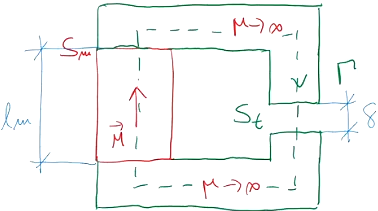
\includegraphics[width = 0.4\linewidth]{magnete_permanente_C}
\end{figure}

Il giogo a ``C'' è analogo a quelli precedentemente analizzati e alimentati da una 
forza magnetomotrice, analogamente il magnete permanente è sede di correnti
molecolari di superficie, che lo percorrono in modo del tutto analogo alle correnti
magnetizzanti che attraversavano gli avvolgimenti negli esempi precedenti.

Si vogliono dunque determinare i parametri geometrici ``ottimi''
del magnete per ottenere un'induzione al traferro $B_t$.
Le dimensioni del magnete sono la sua altezza $l_m$ e la sua sezione $S_m$.

Per la solenoidalità di $\vec{B}$ si può confondere il flusso attraverso il magnete con 
quello attraverso il traferro ed applicare la legge di Ampére ad una liena $\Gamma$.
$B_mS_m = B_tS_t$
$$
\text{f.m.m.} = 0 \text{ su }\Gamma \Rightarrow \vec{H}_ml_m + H_t\delta = 0
$$
le parti in ferro non offrono un forte contributo al campo data l'elevata permeabilità.

Si determinano poi le relazioni costitutive:
$$
B_m = \mathcal{B}\left(H_m\right)\qquad \text{nel magnete}
$$
$$
B_t = \mu_0 H_t\qquad \text{nel traferro}
$$
sostituendo si ottiene:
$$
H_ml_m + \frac{B_t}{\mu_0}\delta = 0 = H_ml_m + \frac{B_mS_m}{S_t\mu_0}\delta
$$
Ossia l'equazione di una retta nel piano $H_m,B_m$.
Quest'ultima va unita alla relazione costitutiva del magnete permanente
$$
B_m = \mathcal{B}\left(H_m\right)
$$
si individua infine il punto di lavoro del magnete permanente mediante un'analisi
matematica delle intersezioni tra le due equazioni, il metodo risolutivo è analogo
a quello utilizzato per i circuiti non lineari.
\begin{figure}[H]
\centering
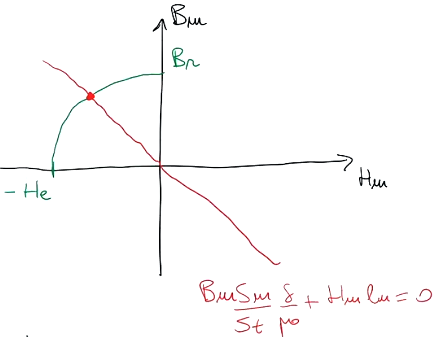
\includegraphics[width = 0.4\linewidth]{intersezione_curva_magnete_permanente}
\end{figure}
Il prodotto $\left|B_mH_mV_m\right|$ rappresenta in un certo senso l'energia immagazzinata
nel magnete permanente, le dimensioni ottime sono quelle che minimizzano il volume del 
magnete.
Conviene stabilire il punto di lavoro in modo che $\left|B_mH_m\right|$ sia massimo,
in modo da minimizzare il volume necessario.

Si possono dunque calcolare le dimensioni $S_m$ ed $l_m$ del magnete.
